\documentclass{beamer}

\usepackage[T1]{fontenc}
\usepackage[utf8]{inputenc}
\usepackage[german]{babel}
\usepackage{multicol}
\usepackage{mathabx}
\usetheme{Warsaw}  %% Themenwahl
\usecolortheme{dolphin}

\title{Präsentation Simulation Drive Trough}

\author{L. Garstenauer S. Steininger S. Wernegger}
\date{\today}
 
\begin{document}
\maketitle
\frame{\tableofcontents[currentsection]}


\section{Aufgabenstellung}
\begin{frame} %%Eine Folie
  \frametitle{Aufgabenstellung} %%Folientitel
	\begin{itemize}
		\item Drive-Through-Schalter, bestehend aus Bestellbereich und Ausgabe
		\item Kunden Erstellung ist abhängig von der Tageszeit
		\item Falls Ausgabeschalter nicht frei ist muss gewartet werden
		\item Kunden können Umkehren wenn Wartezeit zu lang ist
		\item Falls das Essen nicht fertig ist muss darauf gewartet werden.
	\end{itemize}
\end{frame}

\section{Implementierung}
\begin{frame}
	 \frametitle{Implementierung } 
	 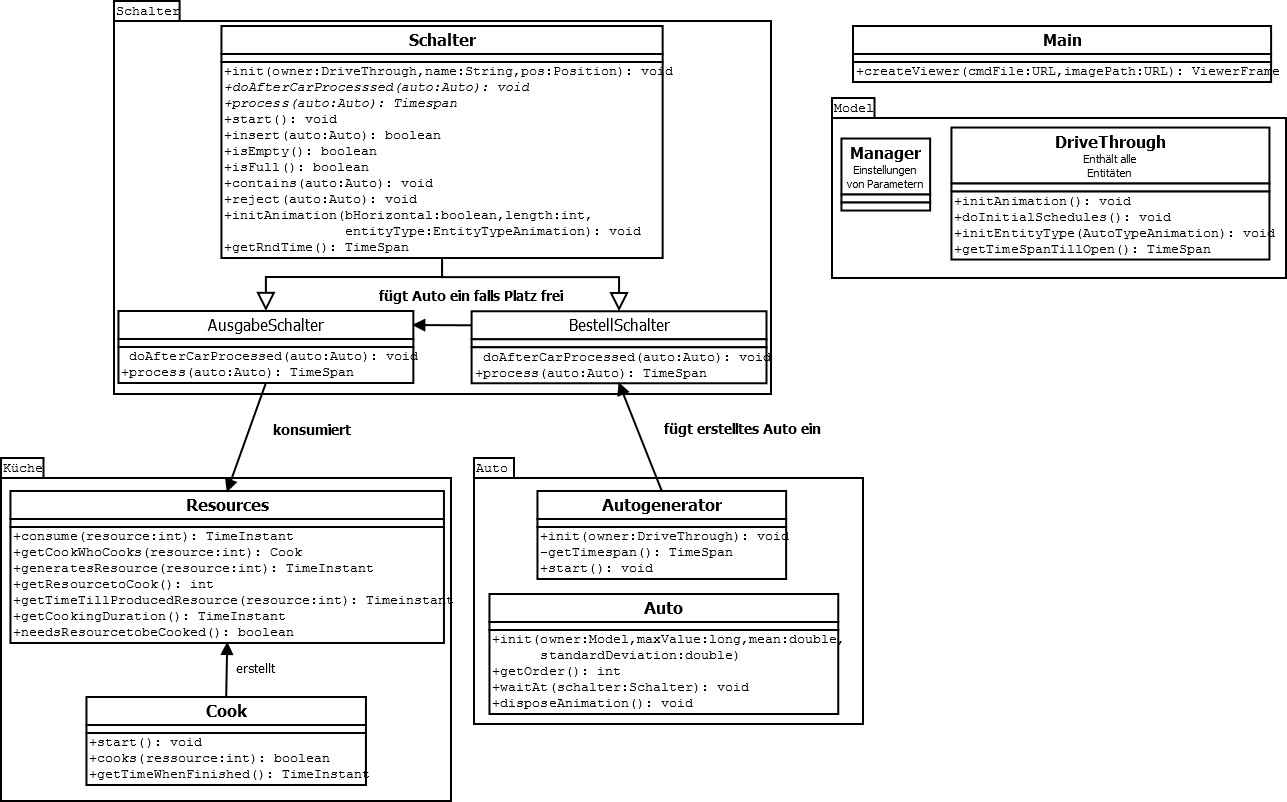
\includegraphics[width=\textwidth]{SimulationUML.png}
	 \begin{itemize}
	 \item []
	 \end{itemize}
	 
\end {frame}


\section{Was wurde getestet?}
\begin{frame} %%Eine Folie
  \frametitle{Was wurde getestet? } %%Folientitel
  Einfluss folgender Parameter auf die Kundenzufriedenheit und Wartezeit
  
 \begin{itemize}
 \item Länge der Warteschlangen Bestellung und Ausgabe
 \item Anzahl der Köche 
 \item Resourcenlimit
 \item Resourcenerstellungsdauer
 \item Anzahl verschiedener Ressourcen
 \item Dauer Bestellung und Ausgabe
 
 \end{itemize}
\end{frame}

\section{Was wurde Beobachtet?}
\begin{frame} %%Eine Folie
  \frametitle{Welche Resultate sind von Interesse } %%Folientitel

  
 \begin{itemize}
 \item Wartezeit im Drive Through gesamt
 \item Wartezeit am jeweiligen Schalter
 \item Durchschnittlicher Ressourcenvorrat
 \item Anzahl der unzufriedenen Kunden
 \item Zeit in der Köche untätig sind
 
 \end{itemize}
\end{frame}




\begin{frame} %%Eine Folie
  \frametitle{Kundenerstellungsverteilung } %%Folientitel
  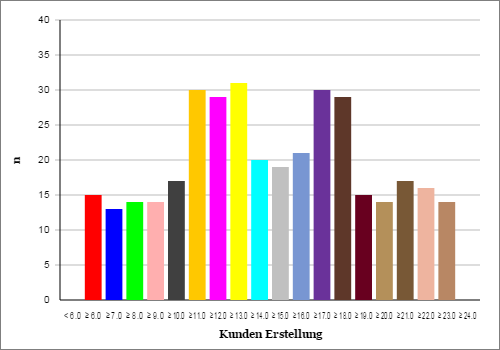
\includegraphics[width=\textwidth, height=0.85\textheight]{./Kunden.png}
 \begin{itemize}
 \item[]
 \item[]
 \end{itemize}
\end{frame}

\section{Ergebnisse}
\begin{frame} %%Eine Folie
  \frametitle{Ergebnisse} %%Folientitel
  \begin{itemize}
  	\item Auswirkungen des Ressourcenerstellung
  	\item Schalterbearbeitungsdauer
  	\item Auslastung der Köche
  \end{itemize}
\end{frame}


\begin{frame} %%Eine Folie
  \frametitle{ Auswirkungen des Ressourcenerstellung} 
  Auswirkung der Veränderung der jeweiligen Parameter
  die bei der Ressourcenerstellung beteiligt sind.\newline
  Veränderte Parameter:
  \begin{itemize}
  	\item Anzahl verschiedener Ressourcen
  	\item Ressourcenlimit erhöht \textbf{+3}
  	\item $\diameter$ Ressourcenerstellungsdauer verringert \textbf{-100 sec}
  	\item Bei einer Anzahl von \textbf{3} Köchen
  \end{itemize}

 
%  \begin{itemize}
 % 	\item Ressourcenstand
  %	\item Unzufriedene Kunden 
  %	\item Wartezeit
  	%\item Auslastung der Köche
 % \end{itemize}

\end{frame} 

\begin{frame}
	Beobachtete alte Werte: \newline 

		%\resizebox{\linewidth}{!}
	
	
	
	\begin{itemize}
	\item[]
	\item Unzufrieden Kunden : 57
	\item Wartezeit bei Ausgabe: $\approx$ 16 min
	\item Auslastung der Köche 100 \%
	\end{itemize}


	 Beobachtete neue Werte: \newline
	
	\begin{tabular}{|l|c|c|c|c|c|}\hline 
     	Ressourcen	&1&2&3&4&5\\ \hline \hline
  	 	Anzahl aller erz. Ress.&65&71&54&60&58\\ \hline
	\end{tabular}
	
	\begin{itemize}
		\item[]
		\item Unzufrieden Kunden : 27
		\item Wartezeit bei Ausgabe: $\approx$ 13 min
		\item Auslastung der Köche 100 \%
	\end{itemize}
	
\end{frame} 

\begin{frame}
	\frametitle{Unzufriedene Kunden } %%Folientitel
  	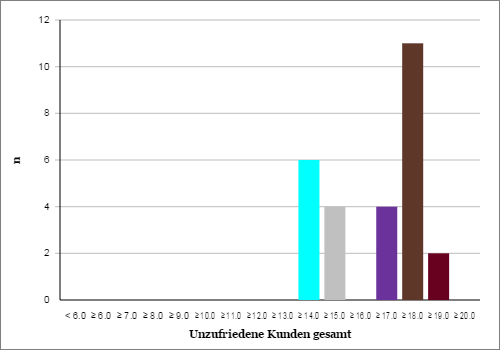
\includegraphics[width=\textwidth, height=0.85\textheight]{./Kundenunzu.png}
 	\begin{itemize}
 		\item[]
 		\item[]
 	\end{itemize}
\end{frame}

\begin{frame} %%Eine Folie
  \frametitle{Schalterbearbeitungsdauer} %%Folientitel
  Einfluss der Bearbeitungsdauer auf die Wartezeit\newline
  Veränderte Parameter:
  \begin{itemize}
  	\item Bestellung- /Ausgabedauer Verhältnis 
  	\item Schalterlänge Ausgabe/Bestellung
  \end{itemize}
  Beobachtete Werte: %%bei folgender Folie auswertung es Reports 
  \begin{itemize}
  	\item Unzufriedene Kunden %Historgamm unzufrieden Kunden 
  	\item Wartezeit % Akkumulate Wartezeit %Queue bestellschater ausgabe zeile Kopieren warteschlange schalterbestellung und ausgabe
  
  	%count Kunde verlässt ausgabe Bestellung
  \end{itemize}
\end{frame}

\begin{frame}

\frametitle{Schalterbearbeitungsdauer-Ergebnisse}
	
	
	Parmeter Zeit am Bestellschalter: 80 sec. \newline
	Parameter Zeit am Ausgabeschalter: 150 sec. \newline
	Beobachtete alte Werte:\newline
	
  	\begin{itemize}
  		\item Anzahl Unzufr. Kunden 9
  		\item $\diameter$ Wartezeit aller Autos $\approx$ 14 min.
  	
  	\end{itemize}

	
	Parmeter Zeit am Bestellschalter: 60 sec. \newline
	Parameter Zeit am Ausgabeschalter: 50 sec. \newline
	Beobachtete neue Werte: \newline
		\begin{itemize}
  		\item Anzahl Unzufr. Kunden 0
  		\item $\diameter$ Wartezeit aller Autos $\approx$ 4 min.
  		
  	\end{itemize}

\end{frame}

\begin{frame}

\frametitle{Schalterbearbeitungsdauer-Ergebnisse}
	
	
	Parmeter Länge Bestellschalter: 7. \newline
	Parameter Länge Ausgabeschalter: 5. \newline
	Beobachtete alte Werte:
	
  	\begin{itemize}
  		\item Anzahl Unzufr. Kunden 9
  		\item $\diameter$ Wartezeit aller Autos $\approx$ 14 min.
  		\item Konsumierte Resourcen 333.
  	
  	\end{itemize}


	Parmeter Länge Bestellschalter: 10. \newline
	Parameter Länge Ausgabeschalter: 10. \newline
	Beobachtete neue Werte: 
		\begin{itemize}
  		\item Anzahl Unzufr. Kunden 47
  		\item $\diameter$ Wartezeit aller Autos $\approx$ 36 min.
  		\item Konsumierte Resourcen 354.
  		
  	\end{itemize}

\end{frame}

\begin{frame} %%Eine Folie
  \frametitle{Auslastung der Köche} %%Folientitel
	Veränderte Parameter:
  \begin{itemize}
  	\item Anzahl der Köche von 3 auf 4 erhöht
  	\item Anzahl der Köche von 3 auf 6 erhöht
  	\item Anzahl der Köche von 3 auf 1 verringert
  \end{itemize}
  
  Beobachtete Werte:
  \newline
%  \begin{
%  \begin{itemize}
% 	\item Ressourcenstand 
% 	\item Unzufriedene Kunden 
%  	\item Wartezeit
%  	\item Auslastung der Köche %queue unbeschäftige Köche
%  \end{itemize}

	
\begin{tabular}{|l|c|c|c|c|}\hline 
    Anzahl der Köche	& 1 &	 3 &	 4  &	 6\\ \hline \hline
   $\Sigma$ aller erz. Ress.&86&267&332 &  341\\ \hline
   Unzufrieden Kunde &	194 &	59 &18	 &0 \\ \hline
   $\diameter$ Wartezeit Bestellsch. &$ \approx$ 94 min & $\approx$ 18 min  &$\approx$ 16 min &$\approx$ 4,5 min \\ \hline
  $\diameter$  Ausl. d. Köche & 100 \% & 100 \% & $\approx$ 97 \% & $ \approx$ 75 \% \\ \hline
 \end{tabular}
  
\end{frame}

\section{Live - Demo}
\begin{frame} %%Eine Folie
  \frametitle{Live - Demo } %%Folientitel
  \begin{itemize}
  	\item Demonstration der Animation
  	\item Beispiel Report
  \end{itemize}
\end{frame}





\end{document}
